\chapter{Analysis and design of the application}
This chapter describes the architecture of the solution. First section explains the high level overview, while the following sections are dedicated for detailed explication of individual parts.

\section{High level overview}
The solution is based on three level data centric application. The data is stored in relational database. Application server accesses the database performs processing on the data and exposes the data to the client-side applications. Two types of clients can be distinguished.

\begin{itemize}
	\item Mobile and web clients developed by the bank, which are accessing internal services.
	\item Mobile and web clients developed by third party developers and companies, which are accessing the external services protected by OAuth\cite{OAuth11} protocol.
\end{itemize}

\begin{figure}[h]
\begin{center}
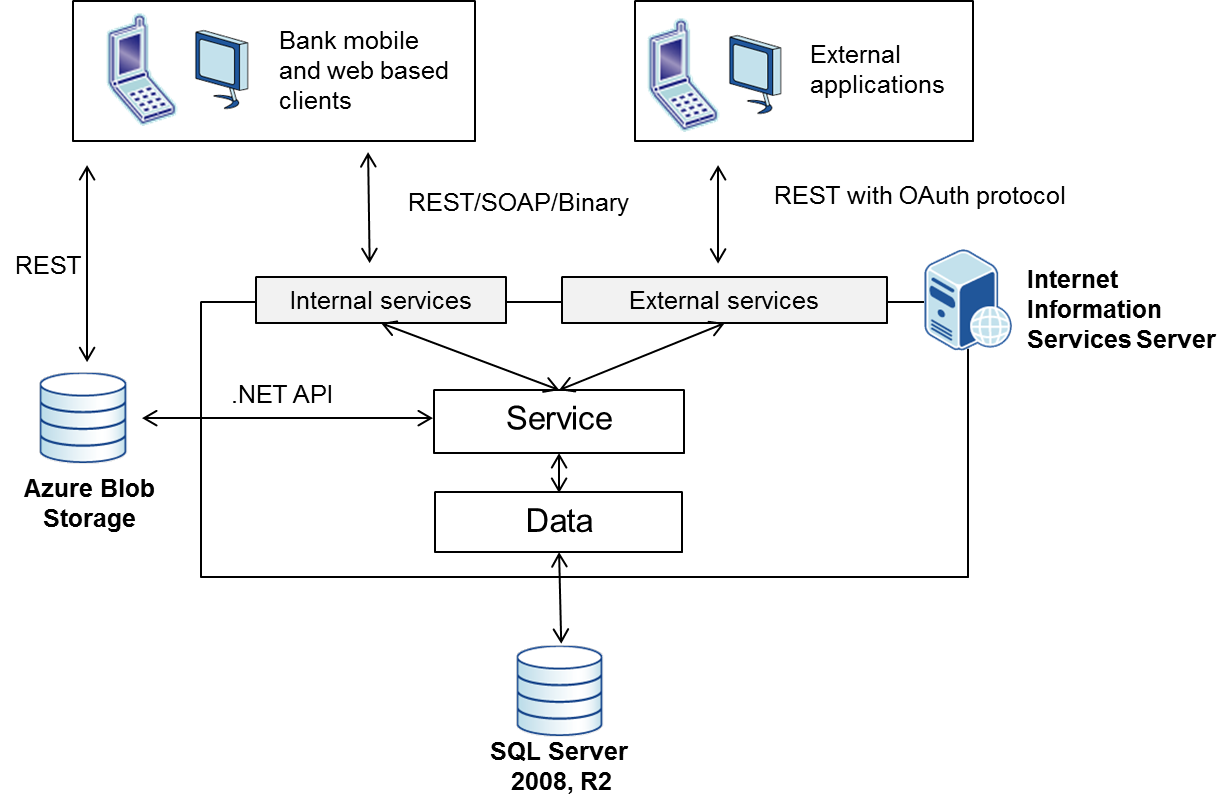
\includegraphics[width=14cm]{figures/big_picture}
\caption{High level overview of the application}
\label{fig:high_level_overview}
\end{center}
\end{figure}

The solution uses secondary non-relational (NoSQL\footnote{While the name suggest that the term refers to databases which are not using SQL language, NoSQL refers to any non-relational type of storage or database.}) storage to implement the "electronic vault" functionality. The client side applications (only the internal ones) can access the NoSQL storage directly. This has the advantage of lowering the throughput and hardware demands on the application server.

In turn the application server also communicates with the NoSQL storage in order to store directly files generated from the banking data. Figure \ref{fig:high_level_overview} summarizes the described situation.

\section{Data access layer}
The data is accessed using Object Relation Mapping (ORM)\cite{wiki:ORM}. Object relational mapping provides the layer between object model represented on the application side and entity model represented on the side of the database. NHibernate ORM framework\cite{NHib09} was chosen for this purpose. See \ref{tech:data} for comparison with other ORM frameworks. Figures \ref{fig:domain_model_1} and \ref{fig:domain_model_2} depict the domain model of the application. Figure \ref{fig:er_model} shows the entity relationship diagram of the database, based on the domain model and created by NHibernate.

Repository pattern is used to encapsulate the data persistence. Repository interfaces define the data access methods which have to be implemented and which are the only way for the business logic to interact with the database. NHibernate persistence logic is used inside the implementation of each repository. Repository pattern thus separates the data access and business layers.

Microsoft SQL Server is used as the main data storage (in the case of on-premise deployment) however the application can use any other database platform compatible with NHibernate. Since the application had to be design to run on Azure platform, the compatibility of NHibernate and Azure SQL was checked.

\section{Business layer}
\label{analysis:business_layer}
Business layer provides the core business methods of the application. As show on figure \ref{fig:appcore}, this layer makes use of the data access layer and serves the data to the communication layer, which later provides the data to several types of client applications.

Business layer is composed of several services. Each of these services concentrates on exposing methods linked with one particular type of application entities. Each service uses Dependency Injection pattern in order to resolve its dependencies specially on Repository implementations.

Dependency Injection allows decoupling of components and moves the responsibility of assembling functional components to external container object. This supports maintainability and modular structure of the project.

There are three cross-cutting concerns which are part of each business class and each business method.

\begin{description}
	\item [Logging] Technical log, which stores the information about the called method, current time and current user. These logs are not meant to be analyzed by business specialist, rather by IT experts.
	\item [Security aspects] Before the execution of each method in the business layer, the system has to determine whether the user has the right to execute the method. This depends not only on the method, but might also depend on the parameters passed to the method.
	\item [Audit trailing] Audit-trail stores the interesting information from business point of view for each significant operation. For instance for making a transfer operation containing debit account, credit account, amount and the initiator of this operation had to be stored. This data should be stored in database in order to allow future simple analysis and also for security purposes.
\end{description}

Aspect oriented programming is used in order to inject the parts of code which implement these concerns into the business methods. Spring.NET is used as Dependency Injection container and cross-cutting concerns injector. Section \ref{tech:di} discusses this choices and other Dependency Injection containers for available for the .NET platform.

\begin{figure}[h]
\begin{center}
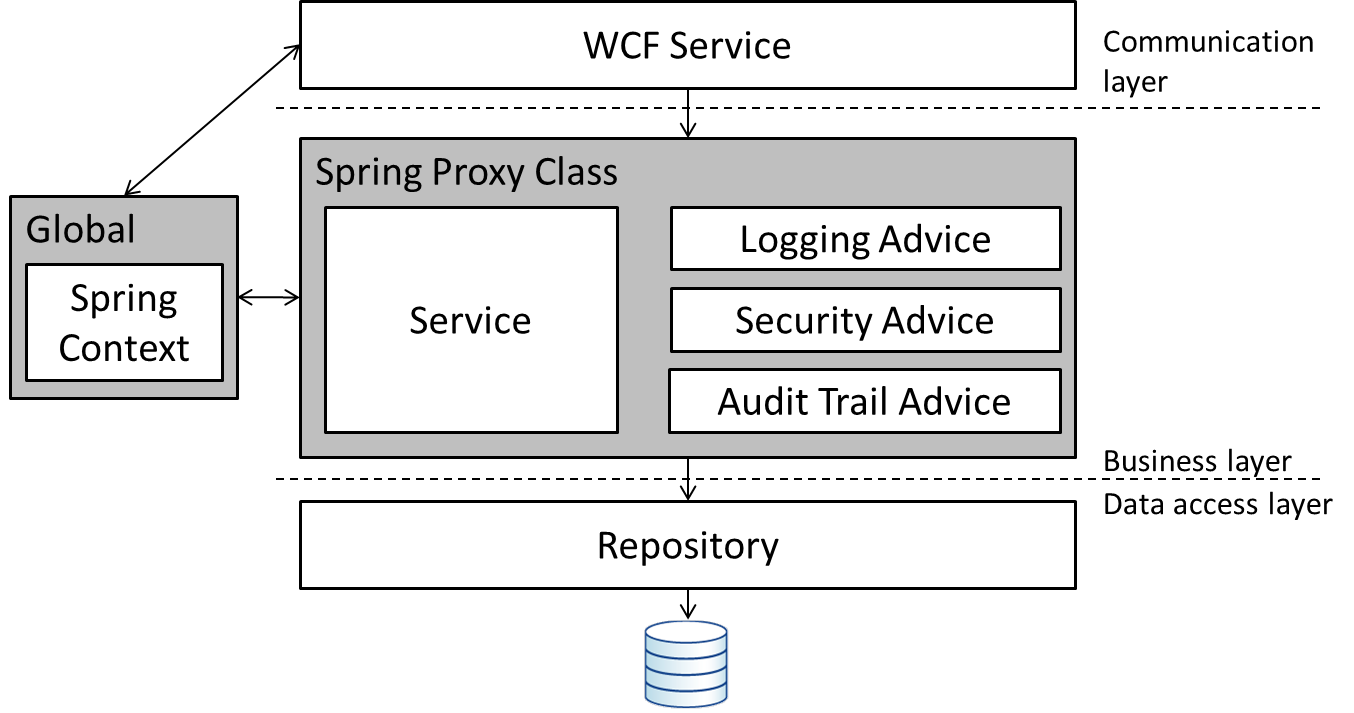
\includegraphics[width=14cm]{figures/business_layer}
\caption{The application core}
\label{fig:appcore}
\end{center}
\end{figure}


\section{Presentation layer}
Presentation layer of this application is heterogeneous. The solution is prepared to support any type of end-user client application. However in the first phase of the implementation two types of clients were implemented: web client and Windows Phone 7 client.

Both of these clients use Silverlight technology as it was required by the requester of this thesis. The standard way of designing Silverlight applications is to use Model View View-Model (MVVM) pattern. This pattern makes use of Silverlight's rich data and command binding options to separate the view from the application logic. Figure \ref{fig:preslayer} shows the usage of MVVM pattern.

The model part contains classes which reflect the server side data model. Concretely the view side model is based on data transfer objects (DTO) which are exposed by server side services.

ViewModels are represented by simple classes which hold the application logic. Each ViewModel encapsulates the logic concerned with concrete application entity. ViewModels also hold the references to the proxies of the server side services. Each ViewModel is thus responsible for getting it's own data.

View is represented by pages and controls written in XAML. XAML is a declarative language used in Windows Presentation Foundation (WPF) and Silverlight, which is used to define the user interface and define the binding between the View and the ViewModel classes.

Thanks to the MVVM pattern we can achieve almost complete separation of view and the the logic behind. As a side effect the logic of the application is isolated in ViewModel classes which are simple C\# classes and can be unit tested. Thus the whole application could run from unit tests.

\begin{figure}[h]
\begin{center}
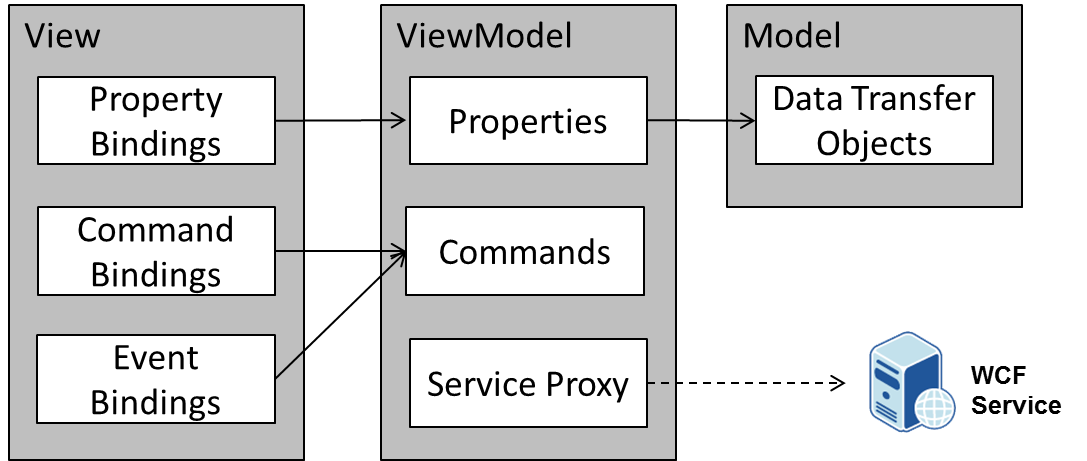
\includegraphics[width=14cm]{figures/presentation_layer}
\caption{Presentation layer}
\label{fig:preslayer}
\end{center}
\end{figure}

\section {Reusing the code between client applications}
In order to minimize the duplication of code in the web and mobile client the solution makes use of Model-View-ViewModel pattern to share the Model and ViewModel parts between both clients. However these two parts are not shared the same way.

The Model part, which contains also proxy classes to access the web service, is compiled as Portable Library project. This type of project makes the compiled assembly usable in all .NET platforms\footnote{The official version of Portable Library project was released on 15 June 2011 supporting .NET Framework, Silverlight, Windows Phone and XBOX platforms}.

The MVVM framework which was developed for this application can be with slight changes compiled for Silverlight and Windows Phone 7 platform. The same code used to define the ViewModels can be used on both platforms, however each project has to reference it's own version of MVVM framework. The solution to this situation is to link the code of the ViewModels between the Silverlight and Windows Phone 7 projects. The whole resulting structure of projects is on Figure \ref{fig:reusable_code}.

\begin{figure}[h]
\begin{center}
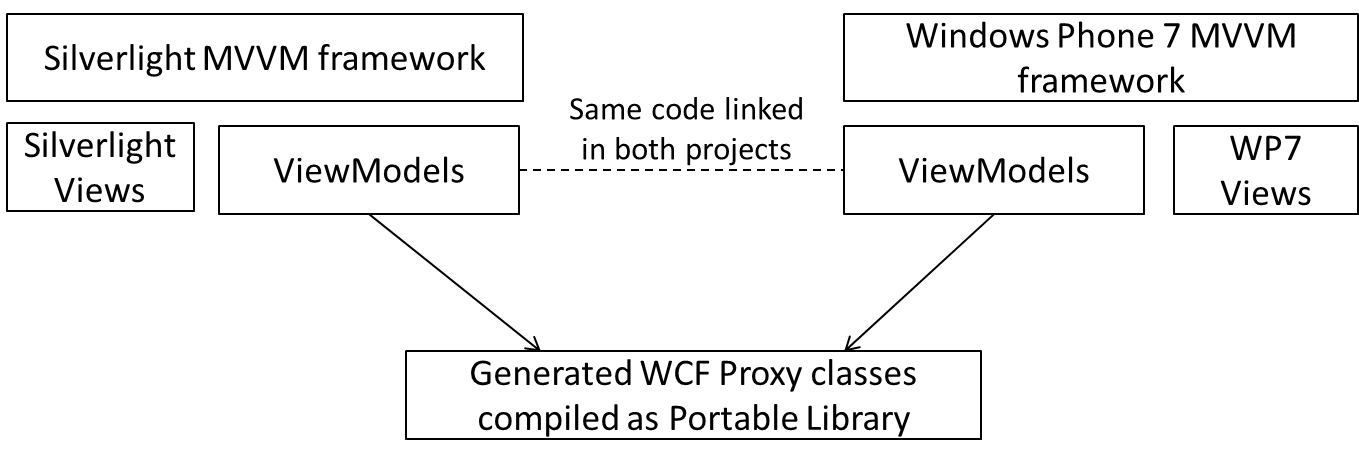
\includegraphics[width=14cm]{figures/reusable_code}
\caption{High level overview of the application}
\label{fig:reusable_code}
\end{center}
\end{figure}

\section{Communication layer}

The application server exposes separated services which provide methods and functions enabling the interaction with the banking system. Each service has a different responsibility.

Two sets of services are provided: the ones for applications developed by the bank and the external services offered for third party developers. Both sets of services are developed using Windows Communication Foundation (WCF). Section \ref{tech:wcf} discusses the main advantages of WCF.

Internal services expose the data using three different transportation formats and protocols. Binary encoding is used to transfer the data between the server and .NET based clients (Windows Phone 7, Silverlight). REST approach using JSON as transformation format is used to expose the data for other mobile clients and traditional SOAP protocol with XML as transportation format is used to enabled web services frameworks of other platforms to easily generate proxy classes (using for example Java Axis or CXF framework).

External services protected using OAuth protocol provide the data in REST-full way with JSON as transportation format.

\section{Integration of non-relational database}
\label{analysis:azureblob}
In the context of this solution a NoSQL database is used to store the client's electronic documents. This is a typical use case for which relational databases introduce higher overhead than NoSQL databases.

\subsection{Structure of Azure Blob Storage}
For this particular case Azure Blob Storage is used to perform the storage of Binary Large Objects (BLOBs). The application accesses the storage using Azure Storage account. Each Azure Storage account can have several containers. In each container several binary large objects can be stored and each blob can be composed of several blocks. Figure \ref{fig:azure_structure} shows the structure of Azure Blob Storage the way it can be used to create an electronic vault for each client.

\begin{figure}[h]
\begin{center}
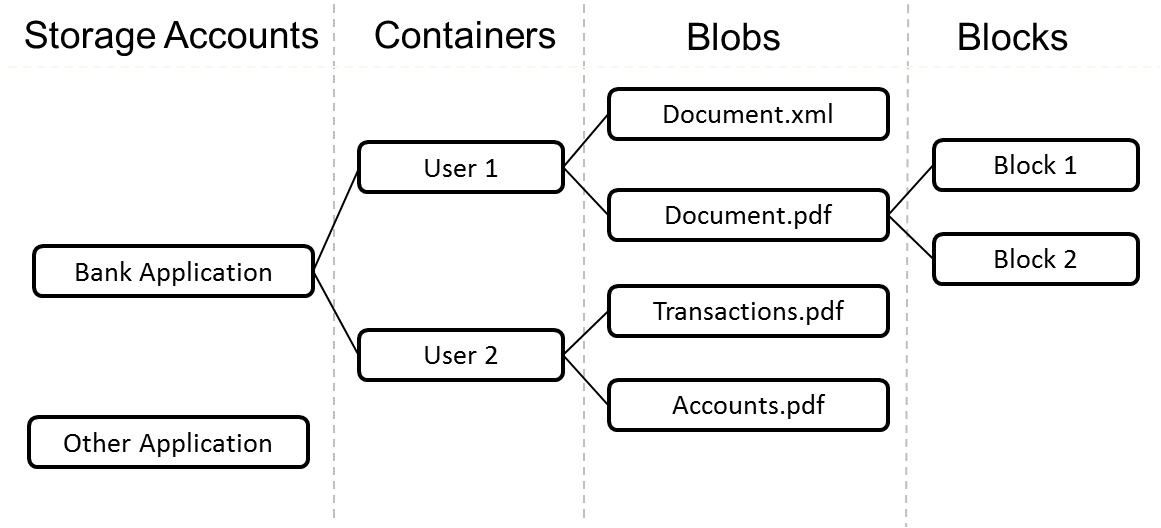
\includegraphics[width=14cm]{figures/azure_storage_structure}
\caption{Structure of Azure Blob Storage}
\label{fig:azure_structure}
\end{center}
\end{figure}

Each client possess one container, which will allow us to assign concrete rights to each container. There is no notion of folders inside of each container, but there is a special naming convention which allows overcoming of this issue.

As seen from the diagram, each file can be separated into several blocks. This is especially useful when treating large files. When file is separated into blocks, than the upload has three phases: first the list of blocks identifications is sent, than each block is uploaded separately and at last a commit is sent to the server. When some of the uploads fail, server can easily send the list of missing blocks to the client. The same applies also to download operations. This separation also allows parallel uploads by several clients.

All blobs are stored in a distributed file system in Azure Fabric\footnote{Azure Fabric is a name given to the network of interconnected computers running Windows Server 2008, which is the base of the Azure platform}. Each blob belongs to one exact partition server. Each blob has a unique key which is composed of its container name and blob name. This key is used as partitioning key, which assigns the blob to one partition server. The access to each partition server is load-balanced and all the partition servers use a common distributed file system. Because each blob has a unique partition key, than in fact the access to each blob is load-balanced, providing good throughput\footnote{In a blog post\cite{azureblob}, which dates May 2010, the Azure Storage Team stated, that the targeted throughput for a single Blob was 60Mb/s. However no other metrics were published since then.}.

\subsection{Application interfaces provided by Azure}
To interact with Azure Storage two possible application interfaces can be used.

\begin{itemize}
	\item .NET Application interface can be used from any .NET assembly running inside Azure cloud platform.
	\item HTTP REST-full Application interface can be used from any application capable of constructing and sending HTTP requests.
\end{itemize}

The access to Azure storage is protected by "storage access key" (Composed of 88 ASCII characters). Every storage account is provided with two keys (called "Primary" and "Secondary") in order to enable renewing of the access keys and keeping zero down time (both of the keys allows access to the storage at the same time).

When using the .NET API, the key is provided to the API which internally uses the key to authenticate the calls to Azure Blog Storage. When using the REST-full API, each HTTP request has to be signed by the key.

On the server side the .NET API can be used to access the storage. The server can store the key encrypted in it's configuration files. In the Silverlight client the only possibility to access the storage is to use the REST-full API. Nevertheless the key is needed to sign the requests.

\section{Security issues}
The access key cannot be given to all Silverlight clients. Silverlight application is merely a collection of files compiled into XAP package, which could be reverse engineered to obtain the key in the case of the access key hard coded inside the package. So the access has to be secured, without giving the access key to the Silverlight client application.

One option would be to build WCF service (secured by SSL) which Silverlight could ask to obtain the access key after performing authentication against the server. However this way the key would be handed to all the clients and once the attacker would infiltrate only one client machine he would also obtain non-restricted access to the whole storage account.

The second option which resolves this issue is to use Shared Access Signatures. Shared Access Signature (SAS) is a temporal authentication token which enables access to concrete blob (or whole container). This way when the client desires to access the storage, it will first contact the server and ask for Shared Access Signature. Server knowing the right information (the demanded blob or container) and being sure that the client is identified will generate the token. This token is then sent to the client using secured channel. The client can than add this token to its upload or download request which will permit him to access the demanded files. Figure \ref{fig:azure_communication} illustrates the communication between client, server and Azure Blob Storage.

\begin{figure}[h]
\begin{center}
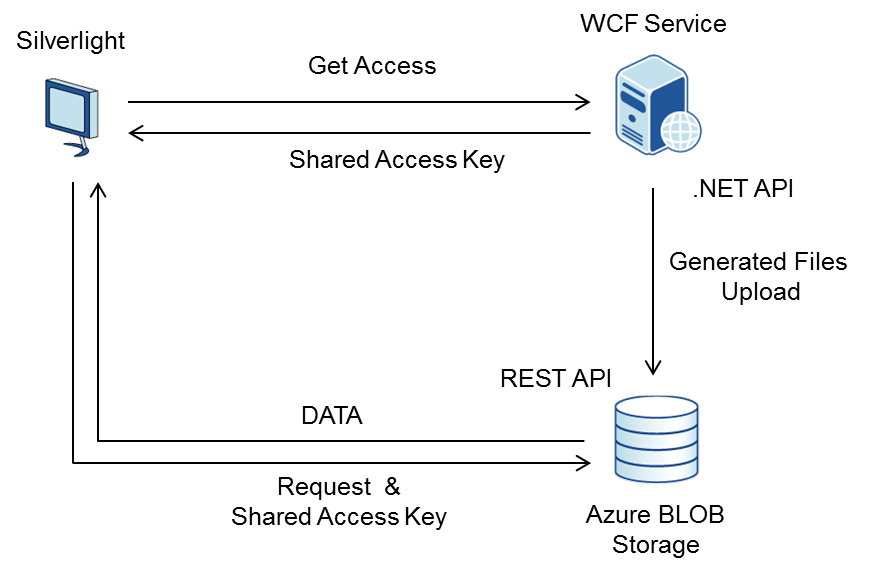
\includegraphics[width=14cm]{figures/azure_storage_calls}
\caption{Secured communication with Azure Blob Storage}
\label{fig:azure_communication}
\end{center}
\end{figure}

Even if the attacker would obtain the Shared Access Signature, the potential danger of misuse would be much lower for two reasons:

\begin{itemize}
	\item Shared Access Signature is a temporal token, valid only during limited period of time.
	\item The attacker would obtain the access just to one container or blob, not the access key which can be used to sign all requests.	
\end{itemize}

\section{Payment categorization}
\label{analysis:payment_categorization}
Automatic payment categorization uses machine learning methods to classify the transactions based on their characteristics. Each transaction has three characteristics (characteristics are sometimes referred to as features) which might be used:

\begin{itemize}
	\item  Date specifies when the transaction was made.
	\item  Amount specifies the sum of the money credited to or debited from the account. For expenses categorization only negative amounts are taken into account.
	\item  Description is a short text which describes the transactions usually originated from Core Banking System. It holds some small amount of meaningful information. For example "\textit{FACTURE CARTE DU 020811 SUPERMARCHE PARIS 06 CARTE 497}" is a short description of payment by card at the supermarket.
\end{itemize}

Out of these characteristics only the "amount" and the "description" can be used during the classification. Even though that the "amount" can hold meaningful information, it is the "description" which will have the biggest impact on the categorization.

Since the description is short text field, payment categorization is based on text categorization. Several types of classifiers can be used to perform text classification such as probabilistic classifiers, decision trees, decision rules, neural networks, example based classifiers or support vector machines \cite{Sebastiani02}.

Naive Bayes classifier does not achieve the best results (in terms of accuracy). However it achieves results comparable to other methods, is fast and relatively easy to implement comparing to more complex methods (such as decision trees, support vector machines or neural networks).\cite{XHemali09} Thus Naive Bayes classifier was chosen to implement the automatic payment categorization.

\subsection{Naive Bayes classifier}
Bayes theorem defines the probability, that an item having features $(F_1,\dots,F_N)$ has category C as\cite{wiki:naiveBayes}:

\begin{equation}
	p(C \vert F_1,\dots,F_n) = \frac{p(C) \ p(F_1,\dots,F_n\vert C)}{p(F_1,\dots,F_n)}. \,
\end{equation}

Since the denominator does not change, only the nominator is used in the probability computation.
Naive Bayes classifier assumes that all features of the classified object are unrelated, thus the conditional probability of an item having features $(F_1,\dots,F_N)$ being of class \textit{C} can be expressed as:

\begin{equation}
	\prod_{i=1}^n p(F_i \vert C)
\end{equation}

Classifier has to work with two types of features: textual (description) and continuous (amount). To enable the usage of textual features, the text has to be converted to binary vector, where each item in the vector corresponds to one word in the dictionary of all the words. If the text description contains the word, the element is set to 1, otherwise to 0.

This enables the conversion of the description of the payment to a set of binary characteristics. Each word is in fact one feature. The text "hello world" can be expressed as a vector \textit{[1,1,0,0]} using the dictionary defined at \ref{tab:word_dictionary}.

\begin{table}
\begin{center}
\begin{tabular}{|c|l|}
\hline
\textbf{index} & \textbf{word} \\
\hline
0 & hello \\
1 & world \\
2 & test \\
3 & new \\
\hline
\end{tabular}
\end{center}
\caption{Dictionary of words}
\label{tab:word_dictionary}
\end{table}

The a priori probability for each category and the conditional probability for each feature category pair have to be estimated. The a priori probability can be simply estimated as:

\begin{equation}
	P(C) = \frac{\# Items Of Category C}{\# Items}
\end{equation}

For the binary features the conditional probability of an item having class C, having feature F can be estimated as:

\begin{equation}
P(F \vert  C) = \frac{\# Items Of Category C Having Feature F}{\# Items Of Category C}	
\end{equation}

In simple terms we are estimating the probability of and item having a certain category when the description contains certain word.

The amount of the payment is continuous characteristic thus traditional Gaussian distribution can be used to estimate the conditional probability of an item having the class C.

\begin{equation}
	P(F = v \vert C) = \frac{1}{\sqrt{2\pi\sigma^2_{c,f}}}\,e^{ -\frac{(v-\mu_{c,f})^2}{2\sigma^2_{c,f}} }
\end{equation}

Before the estimation can be applied the variance ($\sigma^2_{c,f}$) and mean value ($\mu_{c,f}$) have to be computed for each feature-category pair, for all continuous features.

The transactions have to be analyzed before building the model to obtain the parameters for estimation of conditional probability. Concretely the average value and variance has to be obtained for the "amount" of the transaction and the dictionary of words has to be build for the "description" of the transactions.

\subsection{Learning process}
To learn the classifier can use two different sets:

\begin{itemize}
	\item  All categorized transactions of the concerned client.
	\item  All transactions in the system.
\end{itemize}

For most of the clients it will be safe to use all transactions in the system to learn the classifier, however there will be clients having special custom categories or categorizing some transactions in other way than majority of other clients. The wise solution would be to use all transactions only in the situation when there is not enough categorized transactions for each client.

\section{Data interfaces using OAuth protocol}
OAuth protocol is industry standard for delegation of user's rights to third party applications.\cite{OAuth11} It has been developed by cooperation of several engineers of significant internet enterprises\footnote{The group which wrote the initial draft of the protocol was composed of engineers of Google, Twitter, CitizenSpace and Ma.gnolia. The authors of current OAuth draft (version 2.22) are E.Hammer-Lahav Ed (Yahoo), D. Recordon (Facebook) and D.Hardt (Microsoft)}.

OAuth protocol is designed to solve a common situation. The user (or client) is owner of digital resources. To manage his resources the user has to authenticate himself using his credentials. In some situation we can imagine that the client would like to use third party application(s) to manage or use his resources.

Concretely in the banking scenario, the client might like to perform some analytical tasks on the data of his accounts using some third party applications such as Personal Finance Management software.

However to give the application the access to the accounts, he would be forced to share his credentials with the application. This is not desirable while, the application then would obtain full access to all of the resources. Instead using the OAuth protocol, the client can authorize the application to obtain temporal token and access the data using this token. Figure \ref{fig:oauth_workflow} shows the standard OAuth workflow applied to the situation of the bank and the client willing to access his banking data through third party application.

\begin{figure}[h]
\begin{center}
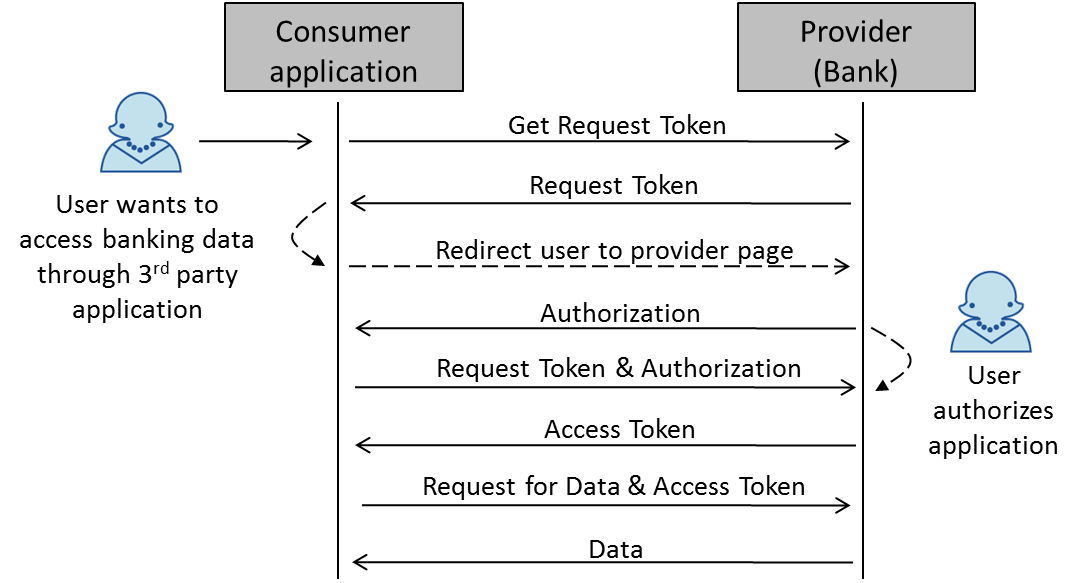
\includegraphics[width=14cm]{figures/oauth_workflow}
\caption{Workflow of the OAuth protocol}
\label{fig:oauth_workflow}
\end{center}
\end{figure}

OAuth protocol uses standard cryptographic tools such as hashing or RSA encryption to secure the HTTP requests and thus encrypting the communication. There are several existing libraries and frameworks which might be useful to facilitate the task of implementation of this protocol. Thanks to the wider possible usage most of these frameworks offer only client side OAuth implementation. There is only one library in the .NET ecosystem, which provides the infrastructure for developing the OAuth provider called DotNetOpenAuth\footnote{\href{http://www.dotnetopenauth.net/}{DotNetOpenAuth} is developed by Andrew Arnott (Microsoft), as an open source project and has been used in several large applications, such as StackOverflow or DotNetNuke}.

DotNetOpenAuth provides classes and methods which enable the developers to easily create OAuth consumer or provider and manipulate tokens. However both consumer and provider have to decide on how to handle and store the tokens and nonces\footnote{Nonce is a cryptography term describing number used only once. In OAuth protocol the nonces are used to evict replay attacks. Both nonces and tokens have to be persisted by the provider}.

The simplest architecture consists of a WCF service which returns the data and is secured by OAuth protocol. Consumer can access this services only when he obtains authorization of the actual user and owner of the resources and if he adds the negotiated token to the request. To obtain the token the consumer has to perform the OAuth "handshake" with OAuth endpoints. Figure \ref{fig:oauth_composition} shows the architecture of OAuth provider implemented using DotNetOpenAuth library.

\begin{figure}[h]
\begin{center}
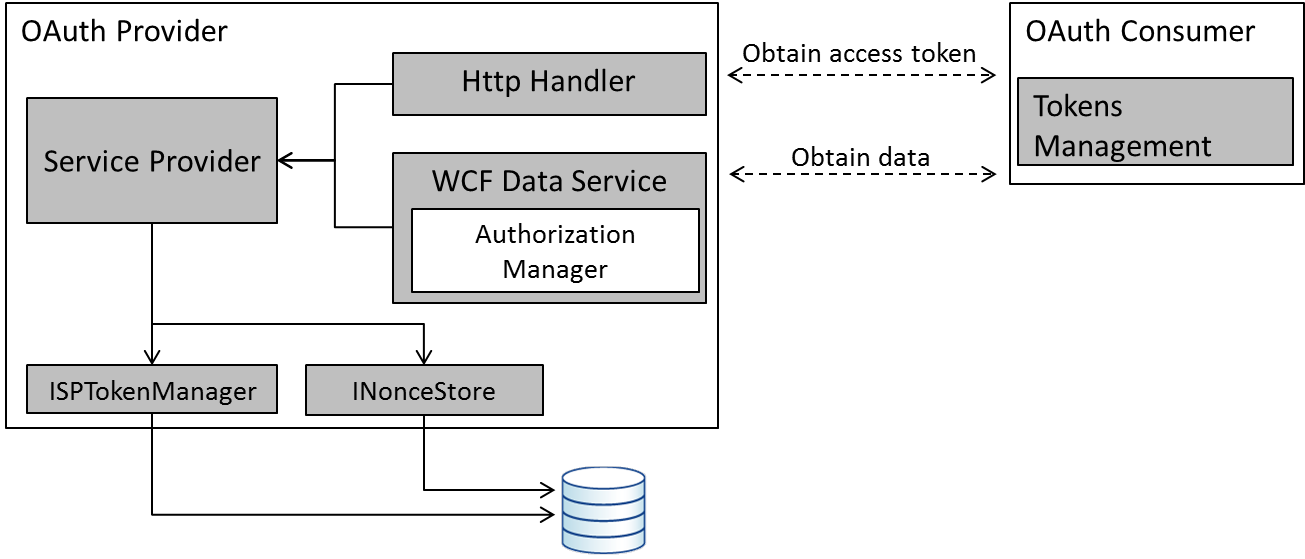
\includegraphics[width=14cm]{figures/oauth_composition}
\caption{The architecture of OAuth provider}
\label{fig:oauth_composition}
\end{center}
\end{figure}

There are two entities which perform the communication. First it is a HTTP Handler which takes care of the OAuth "handshake". The second is the actual WCF service which uses custom Authorization Manager\footnote{Authorization Manager is a WCF message interceptor, which enables definition of custom logic to decide whether the request has passed the authorization or not.} to perform the authentication. Both of these make use of the \textit{ServiceProvider} class, which is a standard part of DotNetOpenAuth library. \textit{ServiceProvider} uses implementations of \textit{IServiceProviderTokenManager} and \textit{INonceStore} also defined in DotNetOpenAuth, which take care of the persistence of nonces and tokens. It is up to the programmer to decide how to implement these interfaces.

The OAuth specification defines four endpoints. \textit{Request}, \textit{Authorize} and \textit{Access} endpoints are used to perform the handshake. The proposed architecture however proposes only one HTTP Handler to perform the handshake. That is because the handler can determine which role to take according to the incoming request. The forth endpoint is the data service.

\subsection{Persistence of OAuth entities}
Since the information about tokens, consumers and nonces have to be stored in the database, these entities have to be added to the application domain and configured to be persisted using NHibernate. 

DotNetOpenAuth already defines the infrastructure in the means of \textit{INonceStore} and \textit{IServiceProviderTokenManager} which in fact are similar to database repositories and interfaces \textit{IServiceProviderRequestToken} and \textit{IServiceProviderAccessToken} which are entities representing the tokens.

The core domain of the application is library independent and all classes are defined as poor old CLR classes. For that reason it would not be advisable to let the POCO objects in the domain implement the DotNetOpenAuth interfaces directly.

Instead of that the DotNetOpenAuth works with classes implementing the DotNetOpenAuth interfaces and these classes are wrappers for the database entities, which in fact do not implement any interfaces. This assures that the core domain of the application would not have to change if there would be different library used for the handling of OAuth protocol. Figure \ref{fig:oauth_wrapping} depicts the classes implementing DotNetOpenAuth interfaces.

\begin{figure}[h]
\begin{center}
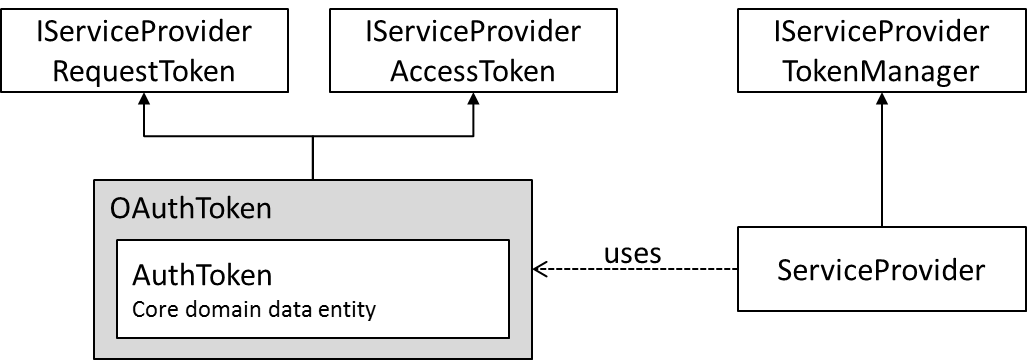
\includegraphics[width=14cm]{figures/oauth_wrapping}
\caption{Classes implementing DotNetOpenAuth interfaces}
\label{fig:oauth_wrapping}
\end{center}
\end{figure}